%!TEX root = ../widefieldscan.tex
%\documentclass{article}
%\usepackage[pdftex,active,tightpage]{preview}
%\usepackage{tikz}
%\usepackage{pgfplots}
%\usetikzlibrary{plotmarks}
%\begin{document}
%\begin{preview}
%%%%%%%%%%%%%%%%%%%%%%%%%%%%%%%%%
	\tikzstyle{every picture}+=[remember picture]
	\tikzstyle{na} = [baseline=-.5ex]
	\begin{flushleft}
	Central Scan \tikz[na] \coordinate (central);
	\end{flushleft}
	%\newline
	Ring Scan \tikz[na] \coordinate (ring);
	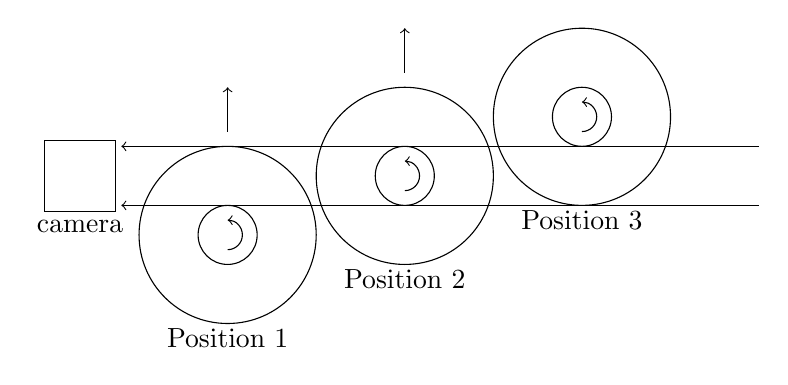
\begin{tikzpicture}[scale=.75]
		%drawing grid
%		\draw[color=gray] (0,0) grid (10,1);
		%camera
			\draw (-.1,-.1) rectangle (1.1,1.1);
			\draw (.5,-.35) node {camera};
		% sample positions
			\foreach \x in {1,2,3}{
				\draw     (3*\x,\x-1.5) circle (.5) circle (1.5);
				\draw[->] (3*\x,\x-1.75) arc (-90:90:.25);
				\draw     (3*\x,-3.25+\x) node {Position \x};
				}
		% movement		
			\foreach \x in {1,2}{				
			    \draw[->]  (3*\x,0.25+\x) -- (3*\x,1+\x);
		% beam
				\draw[<-] (1.2,\x-1) -- (12,\x-1);
				}
		 \path	(3,- .5) coordinate (1-c)
		 		(3,-1.5) coordinate (1-r)
		 		(6,  .5) coordinate (2-c)
		 		(6,- .5) coordinate (2-r)
		 		(9, 1.5) coordinate (3-c)
		 		(9, 0.5) coordinate (3-r);
	\end{tikzpicture}
	\begin{tikzpicture}[overlay]
			\path[->,gray] (central) edge [bend left] (1-c) edge [bend left] (2-c) edge [bend left] (3-c);
    	    \path[->,gray] (ring)    edge [bend right] (1-r) edge [bend right] (2-r) edge [bend right] (3-r);
	\end{tikzpicture}
%%%%%%%%%%%%%%%%%%%%%%%%%%%%%%%%%
%\end{preview}
%\end{document}